% --- ETUDE DE CAS ---
\newpage
\section*{Étude de cas~: ADDS}
\addcontentsline{toc}{section}{Étude de cas~: ADDS}

\section*{AAV}
\addcontentsline{toc}{section}{AAV}
\begin{itemize}
	\item [3] Préparer des scripts PowerShell
    \item [4] Détecter l'annuaire comme le "cœur" du Système d'Information
    \item [3] Schématiser le Système d'Information à l'aide d'un logiciel adapté
    \item [5] Organiser les espaces utilisateurs
    \item [5] Organiser l'arborescence d'un annuaire au regard des bonnes pratiques
    \item [3] Expérimenter la mise en place et la configuration d'Active Directory
    \item [2] Distinguer les niveaux fonctionnels
    \item [3] Préparer des scripts PowerShell permettant d'interagir avec l'AD
    \item [3] Utiliser les stratégies de Groupe
    \item [3] Utiliser les stratégies d'Audit et de sécurité
    \item [2] Différencier les rôles FSMO
    \item [3] Expérimenter la mise en place et la configuration d'un annuaire
    \item [3] Expérimenter la mise en place et la configuration d'un annuaire
    \item [2] Identifier les architectures distribuées et annuaires
\end{itemize}

\newpage

\subsection*{Mots clés}
\phantomsection
\addcontentsline{toc}{subsection}{Mots clés}
\begin{itemize}
	\item Active Directory (AD)
	\item Forêt
	\item Domaine
	\item Rôles FSMO
	\item Relation d'approbation
	\item GPO
	\item NTLM / Kerberos
	\item AGDLP
	\item Niveau fonctionnel
	\item TPE
	\item NTFS
	\item Relation bidirectionnelle
	\item Contrôleur de Domaine
	\item SSO
	\item RODC
	\item LDAP
	\item Diagramme de réseau logique
\end{itemize}

\subsection*{Contexte}
\phantomsection
\addcontentsline{toc}{subsection}{Contexte}
\noindent L'entreprise BERRIA vient d'acquérir IKASI, une TPE voisine. La direction souhaite une intégration technique rapide pour permettre la collaboration entre les équipes, en attendant une migration complète. IKASI dispose de sa propre infrastructure gérée par un prestataire, mais l'audit initial révèle une sécurité laxiste.

\subsection*{Problématique}
\phantomsection
\addcontentsline{toc}{subsection}{Problématique}
\noindent Comment interconnecter de manière sécurisée le système d'information d'IKASI avec l'Active Directory de BERRIA pour permettre le partage de ressources ?

\subsection*{Contraintes}
\phantomsection
\addcontentsline{toc}{subsection}{Contraintes}
\begin{itemize}
	\item Sécurité
	\item Infrastructure existante
	\item OS
\end{itemize}

\subsection*{Généralisation}
\phantomsection
\addcontentsline{toc}{subsection}{Généralisation}
\begin{itemize}
	\item AD
	\item Protocoles d'authentification
	\item Sécurité des systèmes Windows
	\item Gestion des Identités et des Accès (IAM)
\end{itemize}

\subsection*{Livrables}
\phantomsection
\addcontentsline{toc}{subsection}{Livrables}
\begin{itemize}
	\item Diagramme réseau logique
	\item Diagramme de l'AD cible
	\item Liste des stratégies de groupe (GPO)
	\item Architecture de l'AD
\end{itemize}

\subsection*{Pistes de solutions}
\phantomsection
\addcontentsline{toc}{subsection}{Pistes de solutions}
\begin{itemize}
	\item Mise en place d'une relation de forêt
	\item Configuration DNS
	\item Audit et Hardening
	\item Sécurisation via GPO
	\item Gestion des droits fichiers

\end{itemize}

\newpage

\subsection*{Plan d'actions}
\phantomsection
\addcontentsline{toc}{subsection}{Plan d'actions}
\begin{itemize}
	\item Définir les mots clés
	\item Analyser l’architecture existante (Audit)
	\item Étude comparative des différentes architecture AD et de sécurisation
	\item Élaborer le plan de sécurisation
	\item Mise en place d’une relation de Foret
	\item Concevoir l'architecture d'interconnexion
	\item Produire les diagrammes finaux de migration
	\item Préparer l'argumentaire 
	\item Préparer le rapport final
\end{itemize}

\newpage
\section*{Démarche~: ADDS}
\addcontentsline{toc}{section}{Démarche~: ADDS}


\subsection*{Définition~: Mots clés}
\phantomsection
\addcontentsline{toc}{subsection}{Définition: Mots clés}

\noindent \textbf{Active Directory (AD)}:
Système de gestion des identités et des accès développé par Microsoft pour les environnements Windows, permettant de centraliser l'administration des utilisateurs, des groupes et des ressources réseau.

\noindent \textbf{Fôret}:
Structure hiérarchique dans Active Directory qui regroupe plusieurs domaines partageant un schéma commun

\noindent \textbf{Domaine}:
Unité administrative dans Active Directory qui regroupe des objets tels que des utilisateurs, des groupes et des ordinateurs partageant une base de données commune.

\noindent \textbf{Rôles FSMO}:
Rôles spéciaux dans Active Directory qui sont attribués à des contrôleurs de domaine spécifiques pour gérer des fonctions critiques.

\noindent \textbf{Relation d'approbation}:
Mécanisme permettant à deux domaines ou forêts de faire confiance l'un à l'autre pour l'authentification des utilisateurs.

\noindent \textbf{GPO (Group Policy Object)}:
Ensemble de règles et de configurations appliquées aux utilisateurs et aux ordinateurs dans un domaine Active Directory.

\noindent \textbf{NTLM / Kerberos}:
Protocoles d'authentification utilisés dans les environnements Windows pour vérifier l'identité des utilisateurs.

\noindent \textbf{AGDLP}:
Modèle de gestion des groupes dans Active Directory qui signifie "Account, Global, Domain Local, Permission".

\noindent \textbf{Niveau fonctionnel}:
Paramètre dans Active Directory qui détermine les fonctionnalités disponibles en fonction de la version des contrôleurs de domaine.

\noindent \textbf{TPE}:
Très Petite Entreprise, généralement définie comme une entreprise ayant moins de 10 employés.

\noindent \textbf{NTFS}:
Système de fichiers utilisé par les systèmes d'exploitation Windows, offrant des fonctionnalités avancées telles que la sécurité des fichiers et la gestion des permissions.

\noindent \textbf{Relation bidirectionnelle}:
Type de relation d'approbation où deux domaines ou forêts se font mutuellement confiance.

\noindent \textbf{Contrôleur de Domaine}:
Serveur dans un domaine Active Directory qui gère les demandes d'authentification et les accès aux ressources.

\noindent \textbf{SSO (Single Sign-On)}:
Mécanisme permettant aux utilisateurs de s'authentifier une seule fois pour accéder à plusieurs ressources ou applications.

\noindent \textbf{RODC (Read-Only Domain Controller)}:
Type de contrôleur de domaine dans Active Directory qui contient une copie en lecture seule de la base de données.

\noindent \textbf{LDAP (Lightweight Directory Access Protocol)}:
Protocole utilisé pour accéder et gérer les services d'annuaire, y compris Active Directory.

\noindent \textbf{Diagramme de réseau logique}:
Représentation visuelle de l'architecture réseau, montrant les connexions entre les différents composants et systèmes.

\vspace{0.5cm}

\newpage

\section*{Corbeille d'Excercice}
\addcontentsline{toc}{section}{Corbeille d'Excercice}
\subsection*{Prérequis}
\phantomsection
\addcontentsline{toc}{subsection}{Prérequis}
\noindent
\begin{itemize}
	\item Un serveur Windows Server 2022 avec le rôle Active Directory Domain Services installé (ex. domaine de test : \texttt{MONDOMAINE.LOCAL} — nom libre).
	\item Un poste client Windows 10 connecté au réseau du domaine ou pouvant atteindre le contrôleur de domaine.
	\item Accès avec des privilèges administrateur sur le contrôleur de domaine et sur le poste client pour effectuer les manipulations.
	\item Module ActiveDirectory pour PowerShell disponible (ou RSAT installé sur le poste client) pour exécuter les scripts.
	\item Résolution DNS et connectivité réseau fonctionnelles entre le client et le contrôleur de domaine.
	\item Sauvegardes ou snapshots récents du contrôleur de domaine (fortement recommandés avant toute modification).
	\item Environnement de laboratoire isolé conseillé pour les essais afin d'éviter tout impact en production.
	\item Systèmes et correctifs à jour.
\end{itemize}

\vspace{0.5cm}

\noindent Question~: Donnez la commande Powershell pour créer :
\begin{itemize}
	\item une OU à la racine du domaine p.ex. « TEST\_OU »
	\item une sous OU de cette OU p.ex. « SOUS\_OU », sous OU de « TEST\_OU ».
\end{itemize}

\vspace{0.5cm}

\begin{verbatim}
New-ADOrganizationalUnit -Name "TEST\_OU" -Path "DC=MONDOMAINE,DC=LOCAL"
New-ADOrganizationalUnit -Name "SOUS\_OU" -Path "OU=TEST\_OU,DC=MONDOMAINE
,DC=LOCAL"
\end{verbatim}

\newpage

Question~: Créez l'arborescence suivante à l'aide de Powershell

\noindent MONDOMAINE.LOCAL
\begin{itemize}
	\item PERSONNELS
	\begin{itemize}
		\item SALARIES
		\begin{itemize}
			\item APPRENTIS\_CONTRATS\_PROS
			\item CDD
			\item CDI
			\item HONORAIRES
			\begin{itemize}
				\item TVA
				\item HORS\_TVA
			\end{itemize}
			\item A\_TRAITER\_RH
		\end{itemize}
		\item STAGIAIRES
		\begin{itemize}
			\item MARKETING
			\item INFORMATIQUE
			\item AUTRES
		\end{itemize}
		\end{itemize}
	\item ÉQUIPEMENTS
	\begin{itemize}
		\item ORDINATEURS
		\begin{itemize}
			\item SALARIES
			\begin{itemize}
				\item VIP
			\end{itemize} 
			\item STAGIAIRES
		\end{itemize}
		\item COPIEURS
		\begin{itemize}
			\item GROUPES
		\end{itemize}
		\item SECURITE
		\begin{itemize}
			\item GRP\_SEC\_SALARIES
			\item GRP\_SEC\_STAGIAIRES
		\end{itemize}
		\item DISTRIBUTION
		\begin{itemize}
			\item GRP\_DIS\_PARIS
			\item GRP\_DIS\_LYON
			\item GRP\_DIS\_TOULOUSE
			\item GRP\_DIS\_BORDEAUX
		\end{itemize}
		\item SERVICES
	\end{itemize}
\end{itemize}

\newpage

\begin{verbatim}
New-ADOrganizationalUnit -Name "PERSONNELS" 
-Path "DC=MONDOMAINE,DC=LOCAL"
New-ADOrganizationalUnit -Name "SALARIES" 
-Path "OU=PERSONNELS,DC=MONDOMAINE,DC=LOCAL"
New-ADOrganizationalUnit -Name "APPRENTIS\_CONTRATS\_PROS" 
-Path "OU=SALARIES,OU=PERSONNELS,DC=MONDOMAINE,DC=LOCAL"
New-ADOrganizationalUnit -Name "CDD" 
-Path "OU=SALARIES,OU=PERSONNELS,DC=MONDOMAINE,DC=LOCAL"
New-ADOrganizationalUnit -Name "CDI" 
-Path "OU=SALARIES,OU=PERSONNELS,DC=MONDOMAINE,DC=LOCAL"
New-ADOrganizationalUnit -Name "HONORAIRES" 
-Path "OU=SALARIES,OU=PERSONNELS,DC=MONDOMAINE,DC=LOCAL"
New-ADOrganizationalUnit -Name "TVA" 
-Path "OU=HONORAIRES,OU=SALARIES,OU=PERSONNELS,DC=MONDOMAINE,DC=LOCAL"
New-ADOrganizationalUnit -Name "HORS\_TVA" 
-Path "OU=HONORAIRES,OU=SALARIES,OU=PERSONNELS,DC=MONDOMAINE,DC=LOCAL"
New-ADOrganizationalUnit -Name "A\_TRAITER\_RH" 
-Path "OU=SALARIES,OU=PERSONNELS,DC=MONDOMAINE,DC=LOCAL"
New-ADOrganizationalUnit -Name "STAGIAIRES" 
-Path "OU=PERSONNELS,DC=MONDOMAINE,DC=LOCAL"
New-ADOrganizationalUnit -Name "MARKETING" 
-Path "OU=STAGIAIRES,OU=PERSONNELS,DC=MONDOMAINE,DC=LOCAL"
New-ADOrganizationalUnit -Name "INFORMATIQUE" 
-Path "OU=STAGIAIRES,OU=PERSONNELS,DC=MONDOMAINE,DC=LOCAL"
New-ADOrganizationalUnit -Name "AUTRES" 
-Path "OU=STAGIAIRES,OU=PERSONNELS,DC=MONDOMAINE,DC=LOCAL"
New-ADOrganizationalUnit -Name "ÉQUIPEMENTS" 
-Path "DC=MONDOMAINE,DC=LOCAL"
New-ADOrganizationalUnit -Name "ORDINATEURS" 
-Path "OU=ÉQUIPEMENTS,DC=MONDOMAINE,DC=LOCAL"
New-ADOrganizationalUnit -Name "SALARIES" 
-Path "OU=ORDINATEURS,OU=ÉQUIPEMENTS,DC=MONDOMAINE,DC=LOCAL"
New-ADOrganizationalUnit -Name "VIP" 
-Path "OU=SALARIES,OU=ORDINATEURS,OU=ÉQUIPEMENTS,DC=MONDOMAINE,DC=LOCAL"
New-ADOrganizationalUnit -Name "STAGIAIRES" 
-Path "OU=ORDINATEURS,OU=ÉQUIPEMENTS,DC=MONDOMAINE,DC=LOCAL"
New-ADOrganizationalUnit -Name "COPIEURS" 
-Path "OU=ÉQUIPEMENTS,DC=MONDOMAINE,DC=LOCAL"
New-ADOrganizationalUnit -Name "GROUPES" 
-Path "OU=COPIEURS,OU=ÉQUIPEMENTS,DC=MONDOMAINE,DC=LOCAL"
New-ADOrganizationalUnit -Name "SECURITE" 
-Path "OU=ÉQUIPEMENTS,DC=MONDOMAINE,DC=LOCAL"
New-ADOrganizationalUnit -Name "GRP\_SEC\_SALARIES" 
-Path "OU=SECURITE,OU=ÉQUIPEMENTS,DC=MONDOMAINE,DC=LOCAL"
New-ADOrganizationalUnit -Name "GRP\_SEC\_STAGIAIRES" 
-Path "OU=SECURITE,OU=ÉQUIPEMENTS,DC=MONDOMAINE,DC=LOCAL"
New-ADOrganizationalUnit -Name "DISTRIBUTION" 
-Path "OU=ÉQUIPEMENTS,DC=MONDOMAINE,DC=LOCAL"
New-ADOrganizationalUnit -Name "GRP\_DIS\_PARIS" 
-Path "OU=DISTRIBUTION,OU=ÉQUIPEMENTS,DC=MONDOMAINE,DC=LOCAL"
New-ADOrganizationalUnit -Name "GRP\_DIS\_LYON" 
-Path "OU=DISTRIBUTION,OU=ÉQUIPEMENTS,DC=MONDOMAINE,DC=LOCAL"
New-ADOrganizationalUnit -Name "GRP\_DIS\_TOULOUSE" 
-Path "OU=DISTRIBUTION,OU=ÉQUIPEMENTS,DC=MONDOMAINE,DC=LOCAL"
New-ADOrganizationalUnit -Name "GRP\_DIS\_BORDEAUX" 
-Path "OU=DISTRIBUTION,OU=ÉQUIPEMENTS,DC=MONDOMAINE,DC=LOCAL"
New-ADOrganizationalUnit -Name "SERVICES" 
-Path "OU=ÉQUIPEMENTS,DC=MONDOMAINE,DC=LOCAL"
\end{verbatim}

\vspace{0.5cm}

Question~: L'ordinateur client est dans l'OU « COMPUTERS » par défaut. Sur une console visuelle, déplacer un objet d'une OU à une autre se fait en cliquer/glisser ou en clic droit > déplacer. Mais nous allons le faire en powershell.

\noindent Quelles sont les 3 infos nécessaires pour déplacer notre ordinateur depuis une OU vers une autre OU ?

\begin{itemize}
  \item Le nom de l'ordinateur (ex. : \texttt{PC-01\$})
  \item Le chemin LDAP de l'OU source (ex. : \texttt{OU=COMPUTERS,DC=MONDOMAINE,DC=LOCAL})
  \item Le chemin LDAP de l'OU cible (ex. : \texttt{OU=SALARIES,DC=MONDOMAINE,DC=LOCAL})
\end{itemize}

\vspace{0.5cm}

\noindent Quelle est la commande pour déplacer cet objet ordinateur depuis « COMPUTERS » vers « SALARIES/VIP » ?

\vspace{0.5cm}

\begin{verbatim}
Move-ADObject –Identity “CN=PC-CLIENT,OU=Computers,DC=MONDOMAINE,
DC=LOCAL” -TargetPath "OU=VIP,OU=SALARIES,OU=ORDINATEURS,
OU=EQUIPEMENTS,DC=MONDOMAINE,DC=LAN"
\end{verbatim}

\vspace{0.5cm}

Question~: \textbf{Nous allons maintenant créer des comptes d'utilisateur dans notre domaine.}
\noindent Voici un jeu de données à copier-coller dans un fichier CSV. Écrivez le programme pour créer les comptes des utilisateurs dans votre domaine, avec le mot de passe fourni. Vous avez un exemple de capture d'écran d'une fiche utilisateur remplie.
Vous pouvez arbitrairement tous les mettre dans l'OU SALARIES/HONORAIRES.

\noindent (bonus : ajoutez une colonne pour renseigner dynamiquement l'OU)

\vspace{0.5cm}

\textbf{Jeu de données (1 ligne par compte dans le CSV final)} :

\noindent Prenom;nom;Domaine;SAM;Mot de passe\\
Bruce;WILLIS;mondomaine.local;bwillis;Armageddon\$2012\\
Natalie;PORTMAN;mondomaine.local;nportman;<3\_Leon\_<3\\
Keanu;REEVES;mondomaine.local;kreeves;Matrix1999\%\\
Catherine;ZETA JONES;mondomaine.local;czeta-jones;Haute--Voltige1999\\
Christian;CLAVIER;mondomaine.local;cclavier;Keyboard*102touches\\
Marion;COTILLARD;mondomaine.local;mcotillard;Emilien!13!Marseille\\

\textbf{Solution~:}

\begin{verbatim}
clear-host;
$comptes = Import-Csv -Path "C:\liste.csv"
foreach ($compte in $comptes)
{
$Displayname = $compte.Prenom + " " + $compte.Nom
$UserFirstname = $compte.Prenom
$UserLastname = $compte.Nom
$SAM = $compte.SAM
$UPN = $compte.SAM + "@" + $compte.Domaine
$Password = $compte.Password
$OU = "OU=Utilisateurs,DC=mondomaine,DC=local"
New-ADUser -Name "$Displayname" -DisplayName
"$Displayname" -SamAccountName 
$SAM -UserPrincipalName $UPN -
}
\end{verbatim}

\vspace{0.5cm}

Question~: \textbf{Boite à outils AD.}
\noindent Quelles sont les commandes powershell pour :
\begin{itemize}
	\item Afficher le domaine
	\item Afficher les serveurs de contrôleurs de domaine
	\item Afficher les GPO
	\item Lister tous les utilisateurs contenant 2 L dans leur login (Willis, Cotillard)
	\item Lister tous les groupes
	\item Afficher les informations de la forêt
\end{itemize}

\vspace{0.5cm}

\begin{center}
	\begin{tabular}{|p{0.40\textwidth}|p{0.50\textwidth}|}
	\hline
	Action & \texttt{Commande PowerShell} \\ \hline
	Afficher le domaine & \texttt{Get-ADDomain} \\ \hline
	Afficher les serveurs contrôleurs de domaine & \texttt{Get-ADDomainController -Filter *} \\ \hline
	Afficher les GPO & \texttt{Get-GPO -All} \\ \hline
	Lister tous les utilisateurs contenant "ll" dans leur login & \texttt{Get-ADUser -Filter 'samAccountName -like "*ll*"'} \\ \hline
	Lister tous les ordinateurs & \texttt{Get-ADComputer -Filter * -Properties *} \\ \hline
	Lister tous les groupes & \texttt{Get-ADGroup -Filter *} \\ \hline
	Afficher les infos de la forêt & \texttt{Get-ADForest} \\ \hline
	\end{tabular}
\end{center}

\newpage

Question~: \textbf{Application des droits d'accès}
\noindent Dans une entreprise, il existe un \textbf{partage pour le service Direction} qui contient des fichiers/dossiers sensibles

\noindent Il est bien évident que toute l’entreprise ne doit pas avoir accès à cette ressource mais \textbf{seulement les membres de la Direction}. En revanche, il arrive fréquemment que le directeur, Mr Patrick BOSS, demande à son secrétaire, Laurent JOYEUX, de relire certains de ses documents. Il a donc aussi besoin d’un \textbf{accès à ce partage mais seulement en lecture} car le directeur ne veut pas que ses documents soient modifiés.

\noindent Quels groupes créer et quels droits appliquer ?

\textbf{Indice}:
\noindent Nous avons :
\begin{itemize}
	\item 2 utilisateurs
	\item 2 services différents : Direction et Secrétariat
	\item 1 répertoire accessible pour les 2 services : partage « Direction »
	\item 1 accès en lecture/écriture pour le service Direction
	\item 1 accès en lecture pour le service Secrétariat
\end{itemize} 

Vous devez utiliser la méthode \textbf{AGDLP} pour la gestion des droits.
\begin{itemize}
	\item \textbf{A} = Accounting
	\item \textbf{G} = Global (pour groupe global)
	\item \textbf{DL} = Domain local (pour groupe de domaine local)
	\item \textbf{P} = Permissions (qui s’appliqueront sur des ressources)
\end{itemize}

\vspace{0.5cm}

\noindent \textbf{Solution} :
\begin{itemize}
	\item Créer un groupe global « GRP\_DIR » et y ajouter les membres de la Direction (ex. : Patrick BOSS)
	\item Créer un groupe global « GRP\_SEC\_DIR » et y ajouter les membres du secrétariat (ex. : Laurent JOYEUX)
	\item Créer un groupe de domaine local « DL\_DIR\_RW » et y ajouter le groupe global « GRP\_DIR »
	\item Créer un groupe de domaine local « DL\_DIR\_R » et y ajouter le groupe global « GRP\_SEC\_DIR »
	\item Appliquer les permissions « Lecture/Écriture » sur le partage « Direction » au groupe de domaine local « DL\_DIR\_RW »
	\item Appliquer les permissions « Lecture » sur le partage « Direction » au groupe de domaine local « DL\_DIR\_R »
\end{itemize}

\newpage

Question~: Comment déployer ceci en PowerShell ?

\begin{verbatim}
New-ADGroup -Name "GRP\_DIR" -GroupScope Global 
-Path "OU=GROUPES,DC=MONDOMAINE,DC=LOCAL"
Add-ADGroupMember -Identity "GRP\_DIR" -Members "PBOSS"
New-ADGroup -Name "GRP\_SEC\_DIR" -GroupScope Global 
-Path "OU=GROUPES,DC=MONDOMAINE,DC=LOCAL"
Add-ADGroupMember -Identity "GRP\_SEC\_DIR" -Members "LJOYEUX"
New-ADGroup -Name "DL\_DIR\_RW" -GroupScope DomainLocal 
-Path "OU=GROUPES,DC=MONDOMAINE,DC=LOCAL"
Add-ADGroupMember -Identity "DL\_DIR\_RW" -Members "GRP\_DIR"
New-ADGroup -Name "DL\_DIR\_R" -GroupScope DomainLocal 
-Path "OU=GROUPES,DC=MONDOMAINE,DC=LOCAL"
Add-ADGroupMember -Identity "DL\_DIR\_R" -Members "GRP\_SEC\_DIR"
\end{verbatim}

\newpage

\section*{Analyse et résolution : ADDS}
\addcontentsline{toc}{section}{Analyse et résolution : ADDS}

\subsection*{Analyser l’architecture existante (Audit)}
\phantomsection
\addcontentsline{toc}{subsection}{Analyser l’architecture existante (Audit)}
\noindent Avant d'interconnecter les deux Active Directory, un audit approfondi de l'infrastructure existante d'IKASI est essentiel. Cela inclut l'examen des configurations de sécurité, des politiques de groupe (GPO), des permissions d'accès aux ressources et des pratiques de gestion des utilisateurs. L'objectif est d'identifier les vulnérabilités potentielles et de s'assurer que les normes de sécurité sont respectées avant l'intégration.

\begin{center}
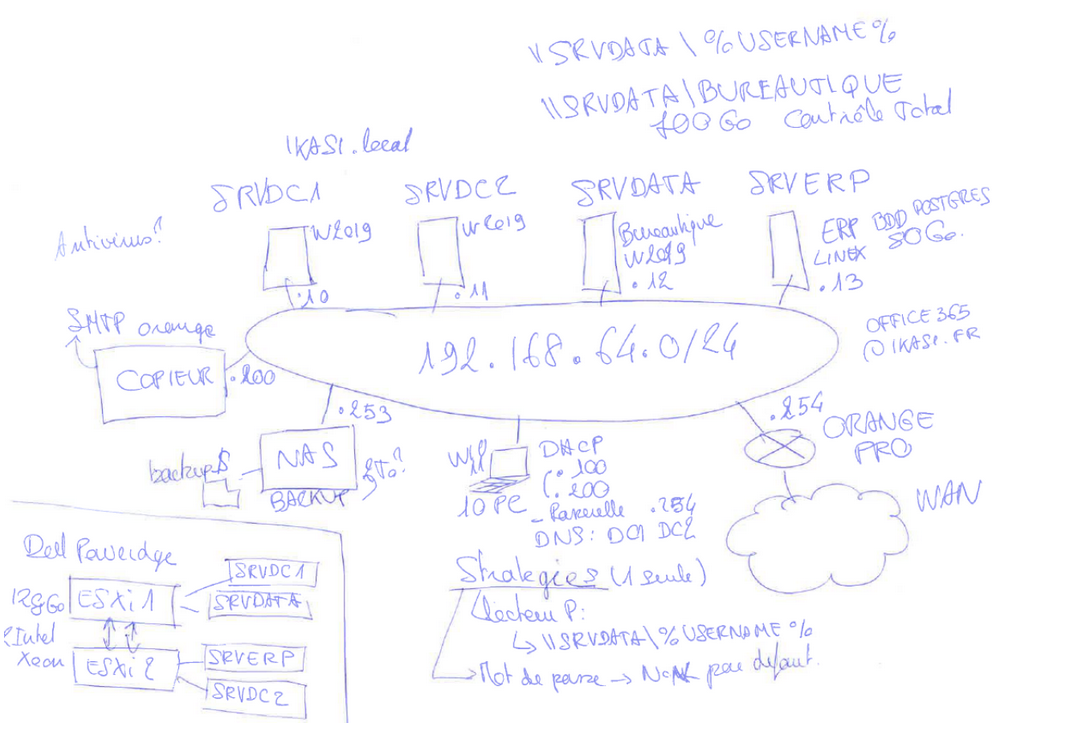
\includegraphics[width=0.7\textwidth]{contents/img/ad_audit.png}
\end{center}

\vspace{0.5cm}

\subsubsection*{Analyse de l'architecture réseau IKASI}
\phantomsection

\paragraph{Infrastructure Principale}
\begin{itemize}
	\item \textbf{Réseau central} : 192.168.64.0/24
	\item Segmentation VLAN implémentée
\end{itemize}

\paragraph{Serveurs Windows (Active Directory)}
\noindent L'infrastructure repose sur \textbf{4 contrôleurs de domaine} :

\begin{enumerate}
	\item \textbf{SRVDC1} — Windows Server 2019, IP : .10
	\item \textbf{SRVDC2} — Windows Server 2019, IP : .11
	\item \textbf{SRVDATA} — Bureautique, Windows Server 2019, IP : .12
	\item \textbf{SRVERP} — ERP + Code Restore 20Go Linux, IP : .13
\end{enumerate}

\newpage

\noindent \textbf{Configuration Active Directory} :
\begin{itemize}
	\item 2 domaines : \texttt{SRVDATA 1 \%USERNAME\%} et \texttt{SRVDATA BUREAUTIQUE 20Go} (contrôle total)
	\item Authentification Kerberos implémentée
	\item Configuration par défaut (Pas de pause → Nom par défaut)
\end{itemize}

\paragraph{Services Réseau}
\noindent \textbf{DHCP} :
\begin{itemize}
	\item Plage d'adresses : 192.168.64.100 à 192.168.64.200
	\item Bail : 10 PC
	\item Passerelle : .254
	\item DNS : 1.0.1 DC2
\end{itemize}

\noindent \textbf{NAS/Backup} :
\begin{itemize}
	\item IP : .253
	\item Fonction : Sauvegarde et stockage réseau
\end{itemize}

\noindent \textbf{Serveur WEB} :
\begin{itemize}
	\item Fonction : Serveur web interne
\end{itemize}

\paragraph{Connectivité Externe}
\noindent \textbf{Routeur/Passerelle} (.254) :
\begin{itemize}
	\item Connexion SHIP Orange vers copieur (200)
	\item Intégration Office 365 (\texttt{IKASI.FR})
	\item Liaison ORANGE PRO (WAN)
\end{itemize}

\paragraph{Réplication Active Directory}
\noindent Architecture de réplication Dell Passerelle :
\begin{itemize}
	\item Rôle : ESXi 1 (Hyperviseur de virtualisation)
	\item Structure hiérarchique :
	\begin{itemize}
		\item SRVDATA $\rightarrow$ SRVDATA (réplication)
		\item ESXi 2 $\rightarrow$ SRVERP + SRVDC2 (sous-jacent Xeon)
	\end{itemize}
\end{itemize}

\paragraph{Points Forts Identifiés}
\begin{itemize}
	\item[\checkmark] \textbf{Redondance} : 4 DC assurent la haute disponibilité
	\item[\checkmark] \textbf{Séparation des rôles} : Serveurs dédiés (ERP, bureautique, données)
	\item[\checkmark] \textbf{Virtualisation} : Infrastructure ESXi pour flexibilité
	\item[\checkmark] \textbf{Sauvegarde} : NAS dédié (.253)
	\item[\checkmark] \textbf{Services cloud} : Intégration Office 365
\end{itemize}

\paragraph{Vulnérabilités et Points d'Attention}
\begin{itemize}
	\item[$\times$] \textbf{Plan d'adressage} : Réseau /24 (254 hôtes max) potentiellement limitant pour l'évolution
	\item[$\times$] \textbf{Sécurité périmétrique} : Absence de DMZ visible pour les services exposés
	\item[$\times$] \textbf{Configuration DHCP} : Plage de 100 IPs pour 10 PC surdimensionnée
	\item[$\times$] \textbf{Documentation} : Relations d'approbation et rôles FSMO peu documentés
	\item[$\times$] \textbf{Audit de sécurité} : Politiques GPO et stratégies d'audit à renforcer
	\item[$\times$] \textbf{Segmentation réseau} : Manque de séparation logique entre services critiques
\end{itemize}

\paragraph{Recommandations Prioritaires}
\begin{enumerate}
	\item \textbf{Documentation des rôles FSMO} : Identifier et documenter clairement les rôles FSMO par DC
	\item \textbf{Mise en place d'une DMZ} : Isoler les services exposés à Internet
	\item \textbf{Stratégies de Groupe (GPO)} : Définir et appliquer des politiques de sécurité strictes
	\item \textbf{Audit de sécurité approfondi} : Évaluer les permissions, les comptes privilégiés et les logs
	\item \textbf{RODC} : Envisager un Read-Only Domain Controller si sites distants
	\item \textbf{Vérification des relations d'approbation} : S'assurer de la configuration correcte entre domaines
	\item \textbf{Plan de reprise d'activité} : Tester régulièrement les procédures de sauvegarde et restauration
\end{enumerate}

\vspace{0.3cm}
\noindent \textit{Cette architecture est typique d'une infrastructure PME avec Active Directory centralisé et virtualisation. L'interconnexion avec BERRIA nécessitera une attention particulière sur la sécurisation et l'harmonisation des politiques de sécurité.}

\newpage

\subsection*{Étude comparative des différentes architecture AD et de sécurisation}
\phantomsection
\addcontentsline{toc}{subsection}{Étude comparative des différentes architecture AD et de sécurisation}
\noindent Plusieurs architectures d'Active Directory et approches de sécurisation peuvent être envisagées. Ci‑dessous un comparatif synthétique, suivi de mesures de durcissement et d'une recommandation pragmatique pour le cas BERRIA / IKASI.

\noindent \textbf{1- Forêt unique — Domaine unique}
\begin{itemize}
	\item Description : Tous les objets (utilisateurs, ressources) dans une seule forêt et un seul domaine.
	\item Avantages : Simplicité administrative, réplication facile, \\ groupes universels, stratégie GPO centralisée.
	\item Inconvénients : Moins d'isolation (exigences légales, politiques divergentes), risque concentré (faille -> impact global).
	\item Cas d'usage : PME ou fusion complète où on accepte une gouvernance commune.
	\item Sécurité : Moins isolé, nécessite un durcissement rigoureux (MFA, LAPS).
\end{itemize}

\noindent \textbf{2- Forêt unique — Domaines multiples}
\begin{itemize}
	\item Description : Une forêt, plusieurs domaines (séparation administrative ou namespace).
	\item Avantages : Isolement administratif et de politique ; conservation d'un schéma commun.
	\item Inconvénients : Complexité de gestion accrue, coûts de réplication, rarement nécessaire pour petites structures.
	\item Cas d'usage : Grandes organisations multi‑régionales ou besoins réglementaires distincts.
	\item Sécurité : Meilleure isolation que domaine unique, mais toujours un point de défaillance unique.
\end{itemize}

\noindent \textbf{3- Forêts multiples avec relations d'approbation (forest trusts)}
\begin{itemize}
	\item Description : Deux (ou plusieurs) forêts séparées liées par des trusts (unidirectionnel/bidirectionnel, sélectif).
	\item Avantages : Forte isolation (schéma, administration), conservation d'autonomie, contrôle fin via selective authentication.
	\item Inconvénients : Complexité DNS/AD DS, gestion des trusts, tests d'interop, limitations sur groupes universels.
	\item Cas d'usage : Fusion temporaire ou collaboration entre sociétés indépendantes (comme BERRIA | IKASI).
	\item Sécurité : Isolation maximale, mais nécessite un durcissement rigoureux des accès inter-forêts.
\end{itemize}

\noindent \textbf{4- Modèle « account forest » / « resource forest »}
\begin{itemize}
	\item Description : Comptes d'utilisateurs dans une forêt, ressources (applications, serveurs) dans une autre ; trusts entre elles.
	\item Avantages : Isolement maximal des ressources, séparation des responsabilités, utile pour hébergeurs/SSO.
	\item Inconvénients : Mise en œuvre complexe (trusts, SID filtering, comptes de service), coûteux pour petites structures.
	\item Cas d'usage : Fournisseurs de services, consolidation d'applications critiques.
	\item Sécurité : Isolation forte, mais nécessite une gestion rigoureuse des accès inter-forêts.
\end{itemize}

\noindent \textbf{5- Architectures hybrides (On-Premises + Azure AD)}
\begin{itemize}
	\item Description : AD on-premises synchronisé avec Azure AD (Azure AD Connect), possibilités de fédération/SSO.
	\item Avantages : Modernisation SSO/MFA, intégration cloud, protection identités (Conditional Access).
	\item Inconvénients : Complexité d'authentification hybride, risques si sync mal configuré, dépendance fournisseur cloud.
	\item Cas d'usage : Entreprises souhaitant utiliser Office365, MFA et services cloud.
	\item Sécurité : Renforcement via MFA, surveillance Azure AD Identity Protection.
\end{itemize}

\noindent \textbf{6- DCs en succursale : RODC / PAW / segmentation}
\begin{itemize}
	\item Description : Read-Only Domain Controllers pour sites distants; \\ postes d'administration dédiés (Privileged Access Workstations).
	\item Avantages : Réduction du blast radius pour sites non sûrs, protection des identifiants administratifs.
	\item Inconvénients : Limitations fonctionnelles (RODC) et coût opérationnel pour PAW.
	\item Cas d'usage : Succursales, sites non maîtrisés ou administrateurs distants.
	\item Sécurité : Renforcement des accès privilégiés, réduction des risques de compromission.
\end{itemize}

\noindent \textbf{Conclusion} : le meilleur compromis pour une PME + TPE est souvent une relation de forêt contrôlée et restreinte, complétée par des mesures de durcissement simples et à fort impact (MFA, LAPS, tiering, audit). Pour des scénarios plus stricts ou multi‑tenants, envisager account/resource forest ou isolation complète avec procédures d'accès fédérés.

\newpage

\subsection*{Élaborer le plan de sécurisation}
\phantomsection
\addcontentsline{toc}{subsection}{Élaborer le plan de sécurisation}
\noindent Le plan de sécurisation doit définir les étapes nécessaires pour renforcer la sécurité de l'Active Directory avant et après l'interconnexion. Cela inclut la mise en œuvre de politiques de mot de passe strictes, la configuration des audits de sécurité, la segmentation des réseaux, et la formation des utilisateurs sur les meilleures pratiques de sécurité. Il est également crucial de définir des procédures de réponse aux incidents pour gérer les éventuelles violations de sécurité.

\vspace{0.5cm}
\textbf{Proposition~:}
\begin{itemize}
	\item \textbf{Mise en œuvre de MFA} : Exiger l'authentification multi-facteurs pour tous les accès administratifs et sensibles.
	\item \textbf{Utilisation de LAPS} : Déployer Local Administrator Password Solution pour gérer les mots de passe des comptes administrateurs locaux.
	\item \textbf{Segmentation réseau} : Isoler les segments critiques (DC, serveurs) avec des VLANs et des pare-feu.
	\item \textbf{Audit et surveillance} : Activer les audits AD, configurer des alertes pour les activités suspectes.
	\item \textbf{Formation des utilisateurs} : Sensibiliser aux risques de phishing, bonnes pratiques de mot de passe.
	\item \textbf{Gestion des accès privilégiés} : Utiliser des comptes dédiés pour l'administration, limiter les droits au strict nécessaire.
	\item \textbf{Plan de réponse aux incidents} : Documenter les procédures en cas de compromission, tests réguliers.
\end{itemize}

\subsection*{Mise en place d’une relation de Foret}
\phantomsection
\addcontentsline{toc}{subsection}{Mise en place d’une relation de Foret}
\noindent La mise en place d'une relation de forêt entre les deux Active Directory nécessite une planification minutieuse. Cela inclut la configuration des relations d'approbation, la synchronisation des DNS, et la vérification de la connectivité réseau entre les deux environnements. Il est également important de tester l'accès aux ressources partagées pour s'assurer que les utilisateurs des deux entreprises peuvent collaborer efficacement tout en respectant les politiques de sécurité établies.

\begin{center}
	\begin{figure}[htbp]
	\centering
	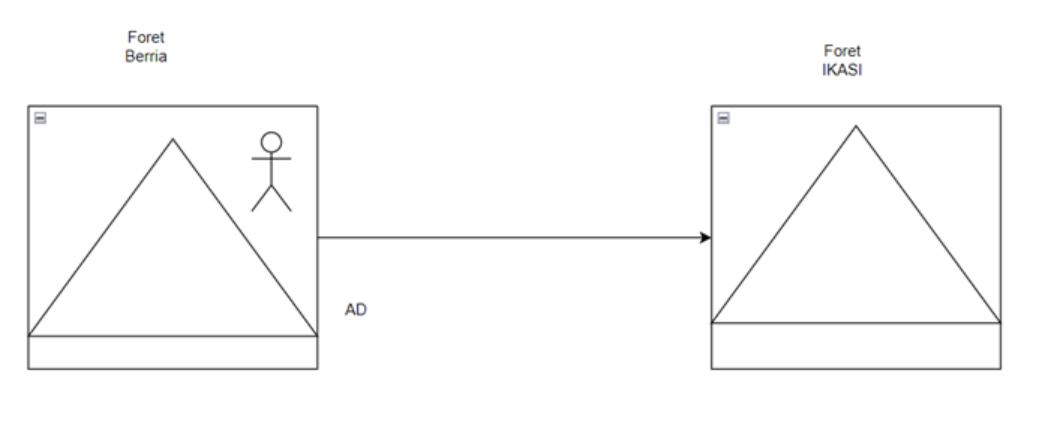
\includegraphics[width=1\textwidth]{contents/img/relation_foret.png}
	\caption{Relation de forêt entre BERRIA et IKASI.}
	\end{figure}
\end{center}

\vspace{0.5cm}

\subsection*{Concevoir l'architecture d'interconnexion}
\phantomsection
\addcontentsline{toc}{subsection}{Concevoir l'architecture d'interconnexion}
\noindent L'architecture d'interconnexion doit être conçue pour garantir une communication sécurisée entre les deux Active Directory. Cela peut inclure l'utilisation de VPN pour sécuriser les connexions, la mise en place de pare-feu pour contrôler le trafic réseau, et l'utilisation de protocoles d'authentification sécurisés tels que Kerberos. Il est également important de documenter l'architecture pour faciliter la gestion et la maintenance future.

\begin{center}
	\begin{figure}[htbp]
	\centering
	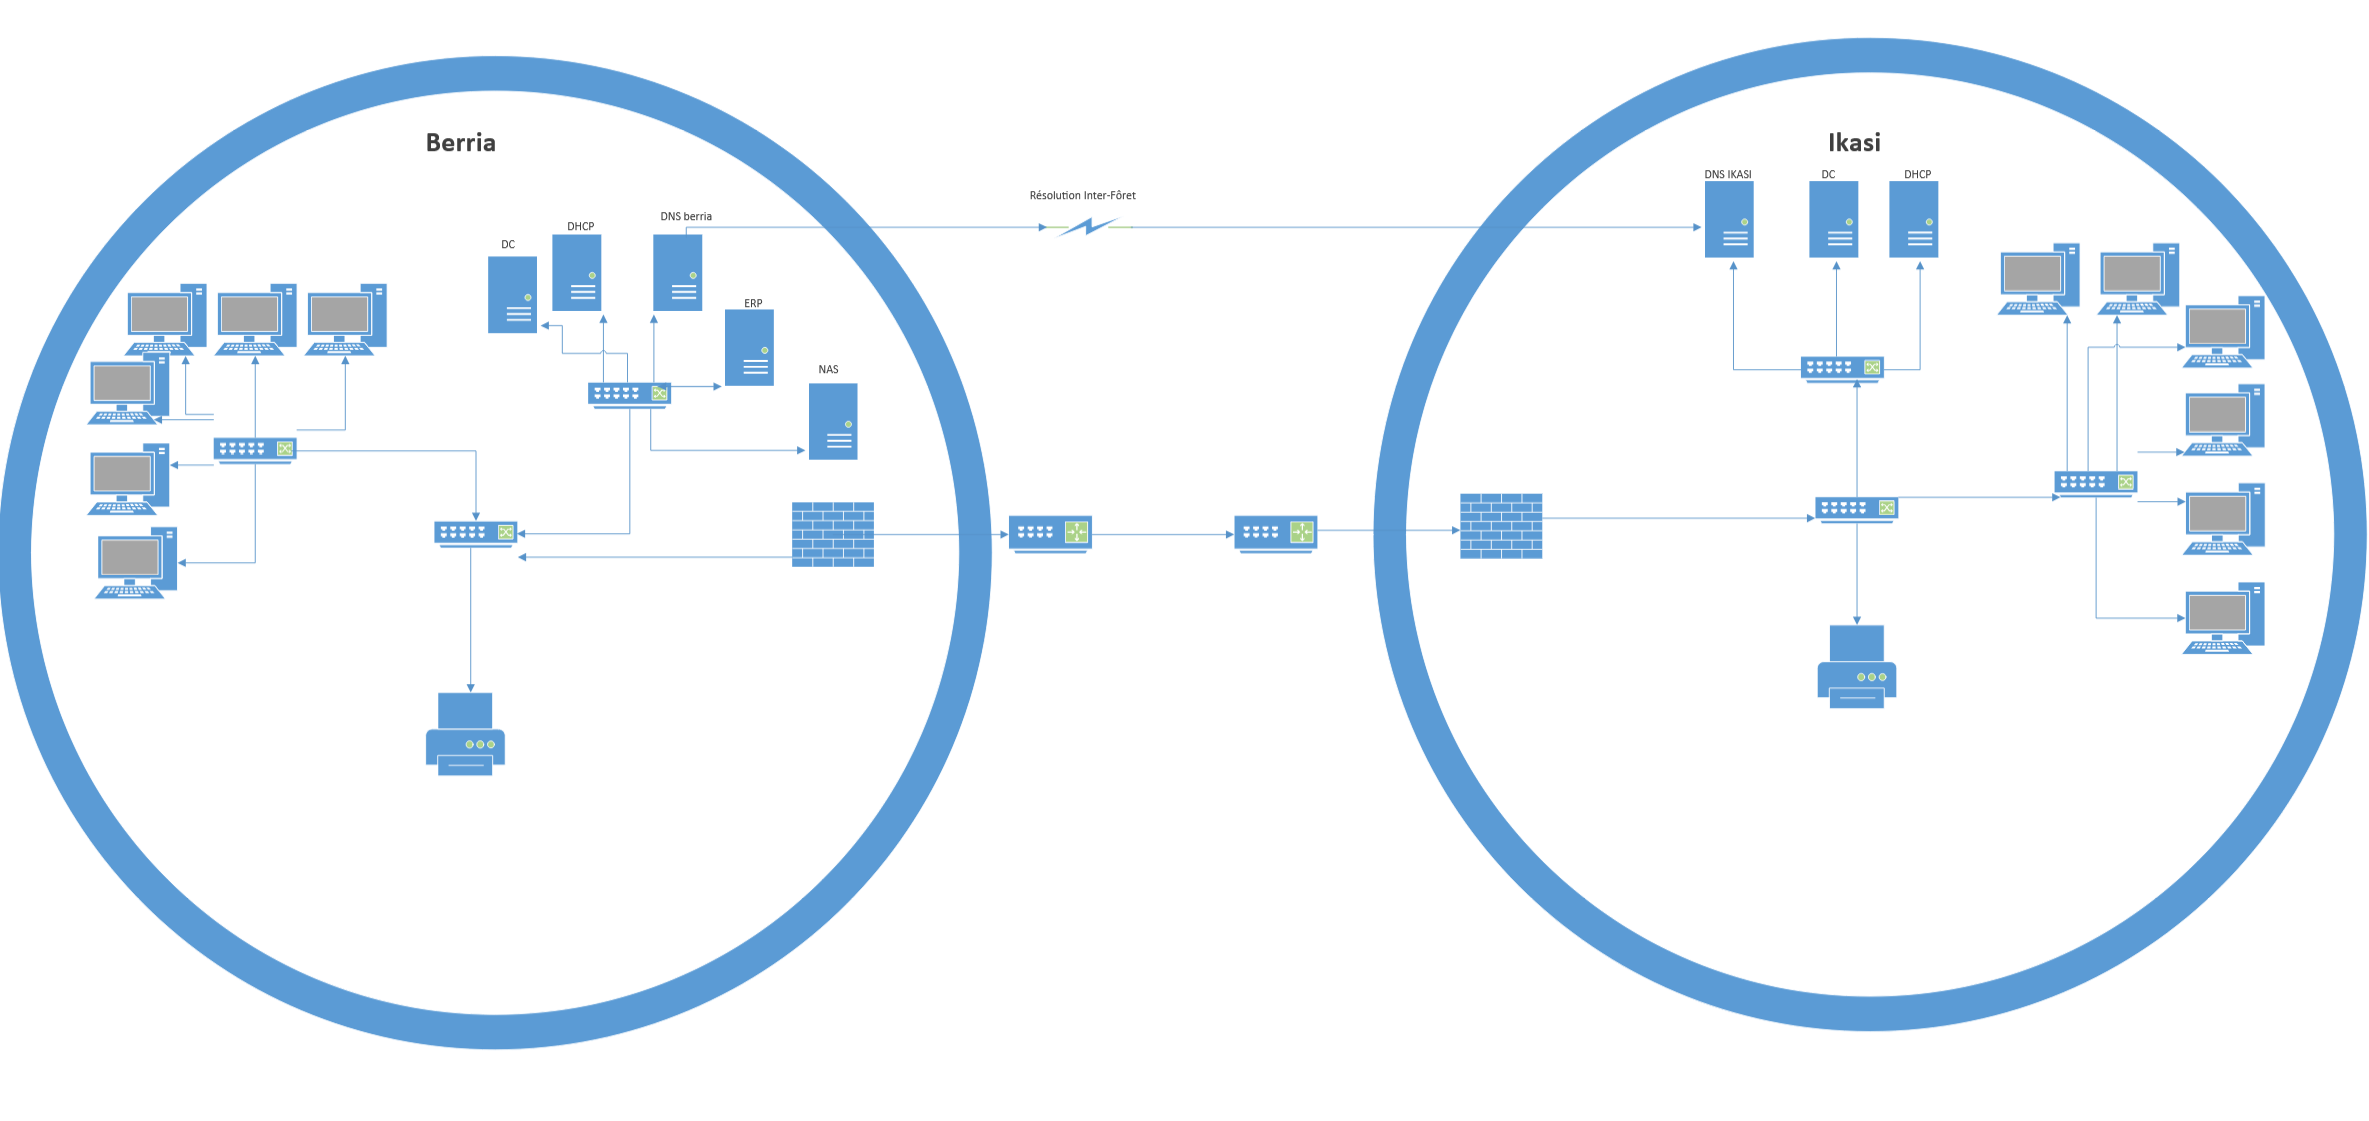
\includegraphics[width=1\textwidth]{contents/img/archi_interconnexion.png}
	\caption{Architecture d'interconnexion entre BERRIA et IKASI.}
	\end{figure}
\end{center}

\begin{center}
	\begin{figure}[htbp]
	\centering
	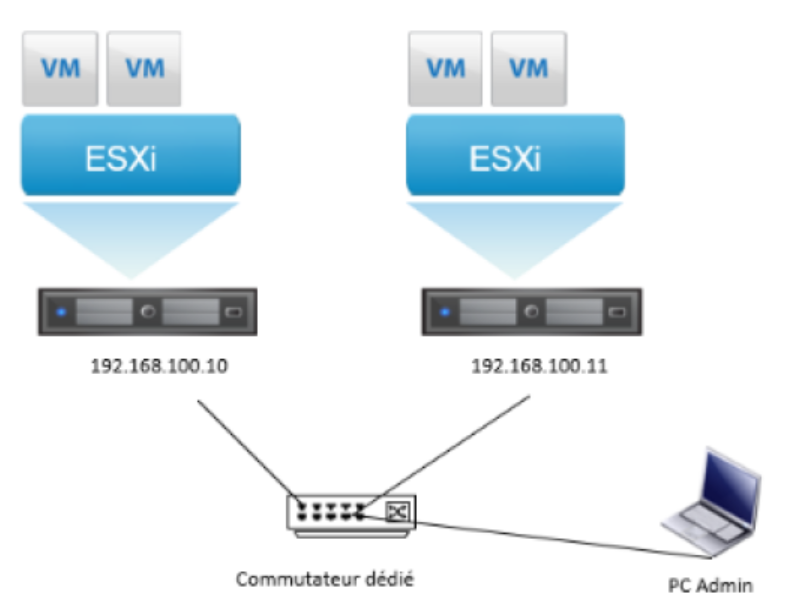
\includegraphics[width=0.5\textwidth]{contents/img/reseau.png}
	\caption{Architecture du reseau externe.}
	\end{figure}
\end{center}

\vspace{0.5cm}

\subsubsection*{Configuration de la haute disponibilité VMware}
\phantomsection

\noindent Pour que les deux serveurs ESXi (192.168.100.10 et 192.168.100.11) puissent fonctionner en relais et assurer la continuité de service des contrôleurs de domaine, plusieurs éléments VMware sont nécessaires :

\paragraph{1. Cluster VMware avec HA (High Availability)}

\noindent \vspace{0.5cm} \\ Le \textbf{High Availability} est une fonctionnalité VMware qui surveille en permanence l'état des hôtes ESXi du cluster. Si un serveur physique tombe en panne, HA redémarre automatiquement les machines virtuelles sur l'autre hôte disponible.

\noindent \textbf{Configuration} :
\begin{itemize}
	\item Créer un cluster vSphere depuis vCenter
	\item Ajouter les deux hôtes ESXi (192.168.100.10 et 192.168.100.11) au cluster
	\item Activer VMware HA dans les paramètres du cluster
	\item Configurer les options de redémarrage des VM (priorité haute pour les DC)
	\item Définir un seuil de tolérance de panne (1 hôte minimum dans ce cas)
\end{itemize}

\noindent \textbf{Avantages} :
\begin{itemize}
	\item Redémarrage automatique des VM en cas de panne matérielle
	\item Temps d'interruption réduit (quelques minutes seulement)
	\item Surveillance proactive de l'état de santé des hôtes
\end{itemize}

\newpage

\paragraph{2. vMotion activé}

\noindent \vspace{0.5cm} \\ \textbf{vMotion} permet de déplacer une machine virtuelle en cours d'exécution d'un hôte ESXi à un autre sans aucune interruption de service. Les utilisateurs ne perçoivent aucune coupure.

\noindent \textbf{Configuration} :
\begin{itemize}
	\item Configurer un réseau vMotion dédié sur chaque hôte ESXi
	\item Activer vMotion sur les adaptateurs réseau appropriés
	\item S'assurer d'une bande passante suffisante (Gigabit minimum, 10Gb recommandé)
	\item Vérifier la compatibilité des CPU entre les deux hôtes
\end{itemize}

\noindent \textbf{Cas d'usage} :
\begin{itemize}
	\item Maintenance planifiée d'un serveur (mise à jour, remplacement matériel)
	\item Équilibrage de charge entre les hôtes
	\item Migration sans interruption de service
\end{itemize}

\paragraph{3. Stockage partagé accessible par les deux ESXi}

\noindent \vspace{0.5cm} \\ Le \textbf{stockage partagé} est essentiel pour que les deux hôtes puissent accéder simultanément aux fichiers des machines virtuelles (VMDK, configuration, snapshots).

\noindent \textbf{Options de stockage partagé} :
\begin{itemize}
	\item \textbf{SAN (Storage Area Network)} : iSCSI ou Fibre Channel
	\item \textbf{NAS (Network Attached Storage)} : NFS
	\item \textbf{vSAN} : Stockage distribué VMware utilisant les disques locaux
\end{itemize}

\noindent \textbf{Configuration (exemple iSCSI)} :
\begin{itemize}
	\item Déployer un serveur de stockage iSCSI (ou utiliser le NAS existant .253)
	\item Créer un LUN partagé pour les VM
	\item Configurer les adaptateurs iSCSI sur chaque ESXi
	\item Monter le datastore partagé sur les deux hôtes
	\item Créer les VM des DC sur ce datastore partagé
\end{itemize}

\noindent \textbf{Importance} :
\begin{itemize}
	\item Permet à vMotion de fonctionner (les fichiers VM restent au même endroit)
	\item Permet à HA de redémarrer les VM sur n'importe quel hôte
	\item Centralise les sauvegardes
\end{itemize}

\paragraph{4. Schéma de fonctionnement}

\noindent \vspace{0.5cm} \\ Avec cette configuration, voici comment le système assure la continuité :

\begin{itemize}
	\item \textbf{Fonctionnement normal} : Les VM (DC) tournent sur l'un des deux ESXi, leurs fichiers sont sur le stockage partagé
	\item \textbf{Maintenance planifiée} : vMotion déplace les VM vers l'autre hôte sans coupure
	\item \textbf{Panne matérielle} : HA détecte la défaillance et redémarre automatiquement les VM sur l'hôte survivant (interruption de 2-3 minutes)
	\item \textbf{Retour à la normale} : Une fois le serveur réparé, on peut redistribuer les VM avec vMotion
\end{itemize}

\vspace{0.3cm}
\noindent \textit{Cette infrastructure de haute disponibilité garantit que les contrôleurs de domaine restent accessibles même en cas de panne d'un serveur physique, assurant ainsi la continuité de l'authentification Active Directory pour BERRIA et IKASI.}

\newpage

\subsection*{Liste des stratégies de groupe (GPO)}
\phantomsection
\addcontentsline{toc}{subsection}{Liste des stratégies de groupe (GPO)}
\noindent Ci‑dessous une liste ciblée de GPO recommandées pour l'interconnexion sécurisée entre BERRIA et IKASI. Chaque GPO est nommée, accompagnée d'un réglage clé et d'une justification opérationnelle. Prioriser tests sur OU pilote avant déploiement global.

\begin{itemize}
	\item \textbf{GPO-Password-Policy} : longueur minimale 12, complexité activée, historique = 24, durée max = 60 jours. (But : réduire le risque par mot de passe.)
	\item \textbf{GPO-Account-Lockout} : seuil = 5, durée de verrouillage = 30 min, reset = 15 min. (But : limiter brute force.)
	\item \textbf{GPO-Kerberos-Hardening} : forcer AES\_256/AES\_128, désactiver RC4, Ticket TGT = 10h. (But : durcir l'authentification entre forêts.)
	\item \textbf{GPO-DC-Baseline} : pare‑feu serveur, désactivation services inutiles, deny interactive logon pour comptes non‑admin. (But : réduire surface d'attaque des DC.)
	\item \textbf{GPO-LDAPS-Only} : forcer LDAPS (636), interdire binds anonymes. (But : chiffrer les échanges d'annuaire entre forêts.)
	\item \textbf{GPO-DNS-Secure} : mises à jour sécurisées, restreindre mises à jour dynamiques. (But : prévenir spoofing DNS entre domaines.)
	\item \textbf{GPO-Trust-SelectiveAuth} : appliquer selective authentication sur comptes utilisés pour trusts, restreindre groupes autorisés. (But : limiter accès cross-forest.)
	\item \textbf{GPO-LAPS} : déployer LAPS + délégation lecture limitée. (But : suppression mots admin locaux statiques.)
	\item \textbf{GPO-Audit-Centralized} : activer audit avancé (success/fail) et forward syslogs/SIEM. (But : détection et traçabilité inter‑forêts.)
	\item \textbf{GPO-SMB-Disable} : désactiver SMBv1, exiger SMB signing. (But : atténuer vulnérabilités SMB.)
	\item \textbf{GPO-Firewall-DC} : n'autoriser que RPC, Kerberos, DNS, LDAPS entre DCs des deux sites. (But : restreindre flux inter‑forêts.)
	\item \textbf{GPO-Workstation-Hardening} : PowerShell execution policy AllSigned, blocage macros non signées, verrouillage session (10 min). (But : réduire vecteurs d'infection côté postes.)
	\item \textbf{GPO-BitLocker} : chiffrement disque obligatoire pour postes et serveurs critiques, gestion clés via AD. (But : protection données au repos.)
	\item \textbf{GPO-Patch-WSUS} : configuration WSUS/maintenance windows et rollback testés. (But : réduire fenetre d'exploitation.)
	\item \textbf{GPO-Governance} : catalogage GPO (nom, owner, description, ticket CHG). (But : tracabilité et gouvernance des changements.)
\end{itemize}

\newpage

\noindent Bonnes pratiques de déploiement :
\begin{itemize}
	\item documenter chaque GPO (nom, portée, responsable, justification, rollback),
	\item déployer d'abord sur OU pilote puis valider impact (test utilisateur, réplication, logs),
	\item appliquer security filtering (retirer Authenticated Users si nécessaire) et délégations minimales,
	\item automatiser export/backup des GPO (Backup-GPO) et versionner les configurations.
\end{itemize}

\noindent Exemples rapides PowerShell (module GroupPolicy) pour créer, lier et sauvegarder des GPOs (adapter les cibles) :

\begin{verbatim}
# créer et lier une GPO au domaine
Import-Module GroupPolicy
New-GPO -Name "GPO-Password-Policy" -Comment "Password policy 
pour le domaine"
New-GPLink -Name "GPO-Password-Policy" -Target "DC=MONDOMAINE,
DC=LOCAL" -LinkEnabled Yes

# définir une valeur registre (ex. verrouillage écran) via GPO
Set-GPRegistryValue -Name "GPO-Workstation-Hardening" -Key 
"HKLM\Software\Policies\Microsoft\Windows\Personalization" 
-ValueName "ScreenSaveTimeOut" -Type Dword -Value 600

# activer audit avancé (ex. Audit Account Logon)
Set-GPRegistryValue -Name "GPO-Audit-Centralized" -Key 
"HKLM\System\CurrentControlSet\Control\Lsa" -ValueName 
"AuditBaseObjects" -Type Dword -Value 1

# restreindre application de la GPO (security filtering) : 
supprimer Authenticated Users, ajouter groupe spécifique
$gpo = Get-GPO -Name "GPO-DC-Baseline"
Set-GPPermissions -Name $gpo.DisplayName -PermissionLevel 
GpoApply -TargetName "DOMAINE\Group_Admins" -TargetType Group
Remove-GPPermission -Name $gpo.DisplayName -TargetName 
"Authenticated Users" -TargetType Group -PermissionLevel GpoApply

# sauvegarder la GPO
Backup-GPO -Name "GPO-Password-Policy" -Path "C:\GPO_Backups"
\end{verbatim}

\noindent Pour l'interconnexion BERRIA <-> IKASI, attention particulière aux GPO liés aux DCs et à la configuration des trusts (Selective Authentication, DNS sûr, LDAPS), tester la réplication et la résolution DNS avant d'ouvrir les accès de ressources.

\subsection*{Conclusion}
\phantomsection
\addcontentsline{toc}{subsection}{Conclusion}
La mise en place d'une architecture de sauvegarde résiliente et souveraine est essentielle pour garantir la continuité des activités face aux menaces croissantes telles que les rançongiciels. En adoptant des stratégies de sauvegarde robustes, en utilisant des technologies adaptées et en automatisant les processus de vérification, les organisations peuvent minimiser les risques de perte de données et assurer une reprise rapide en cas d'incident. La ADDS du système d'information n'est pas seulement une question de technologie, mais aussi de planification, de formation et de vigilance continue.

\newpage

\section*{Capitalisation}
\addcontentsline{toc}{section}{Capitalisation}

\begin{center}
\setlength{\tabcolsep}{10pt}

\begin{tabular}{|p{0.30\textwidth}|p{0.45\textwidth}|m{0.08\textwidth}|}
\hline
\textbf{AAV} & \textbf{Commentaire} & \textbf{Statut} \\ \hline

Préparer des scripts PowerShell &
Exemples fournis (création OU, utilisateurs, groupes, déplacement d'objets). Manque gestion d'erreurs, validation et sécurisation des scripts. &
{\color{orange}Partiel} \\ \hline

Détecter l'annuaire comme le "cœur" du SI &
Rôle central d'AD bien expliqué et illustré par l'audit et les diagrammes. &
{\color{green!60!black}Acquis} \\ \hline

Schématiser le Système d'Information &
Diagrammes présents (réseau, interconnexion) mais normalisation et légendes à améliorer. &
{\color{orange}Partiel} \\ \hline

Organiser les espaces utilisateurs &
OU et espaces utilisateurs définis et appliqués (ex. SALARIES, STAGIAIRES). &
{\color{green!60!black}Acquis} \\ \hline

Organiser l'arborescence d'un annuaire au regard des bonnes pratiques &
Arborescence détaillée et conforme aux bonnes pratiques (AGDLP expliqué). &
{\color{green!60!black}Acquis} \\ \hline

Expérimenter la mise en place et la configuration d'Active Directory &
Déploiement réalisé en laboratoire (DC Windows Server 2019/2022) ; pas de déploiement en production. &
{\color{orange}Partiel} \\ \hline

Distinguer les niveaux fonctionnels &
Niveaux fonctionnels définis théoriquement. &
{\color{green!60!black}Acquis} \\ \hline

Préparer des scripts PowerShell permettant d'interagir avec l'AD &
Scripts d'interaction fournis. &
{\color{green!60!black}Acquis} \\ \hline

Utiliser les stratégies de Groupe &
GPO listées et tests basiques mentionnés ; déploiement et tests avancés manquants. &
{\color{orange}Partiel} \\ \hline

Utiliser les stratégies d'Audit et de sécurité &
Recommandations de durcissement présentes (audit, MFA, LAPS) ; configuration pratique limitée. &
{\color{orange}Partiel} \\ \hline
Différencier les rôles FSMO &
Rôles FSMO expliqués  &
{\color{green!60!black}Acquis} \\ \hline

Expérimenter la mise en place et la configuration d'un annuaire (dup.) &
Tests en labo effectués mais sans scénarios de migration/production complets. &
{\color{orange}Partiel} \\ \hline

Identifier les architectures distribuées et annuaires &
Architectures (forêts, trusts, account/resource) étudiées ; pas de cas pratiques d'interconnexion détaillés. &
{\color{orange}Partiel} \\ \hline

\end{tabular}
\end{center}

\section*{Ressources}
\addcontentsline{toc}{section}{Ressources}

\begin{itemize}
	\item Microsoft Docs — Active Directory Domain Services (AD DS) : \\
	\url{https://docs.microsoft.com/en-us/windows-server/identity/active-directory-domain-services}
	\item PowerShell Documentation — Active Directory Module : \\
	\url{https://docs.microsoft.com/en-us/powershell/module/activedirectory/?view=windowsserver2022-ps}
	\item Pluralsight — Active Directory Fundamentals : \\
	\url{https://www.pluralsight.com/courses/active-directory-fundamentals}
	\item SANS Institute — Active Directory Security : \\
	\url{https://www.sans.org/course/active-directory-security}
	\item YouTube — PowerShell for Active Directory : \\
	\url{https://www.youtube.com/playlist?list=PL6gx4CsQm3aM5Z0f9n0yX6xX6xX6xX6x}
	\item TechNet Gallery — Active Directory PowerShell Scripts : \\
	\url{https://gallery.technet.microsoft.com/scriptcenter/site/search?filter=active%20directory%20powershell}
\end{itemize}
